%(BEGIN_QUESTION)
% Copyright 2006, Tony R. Kuphaldt, released under the Creative Commons Attribution License (v 1.0)
% This means you may do almost anything with this work of mine, so long as you give me proper credit

Gitt væskeflowmåleren og lagringstanken vist her, bestem akkumulert volum i tanken ved de følgende tidspunktene, for strømningsratene vist i grafen:

$$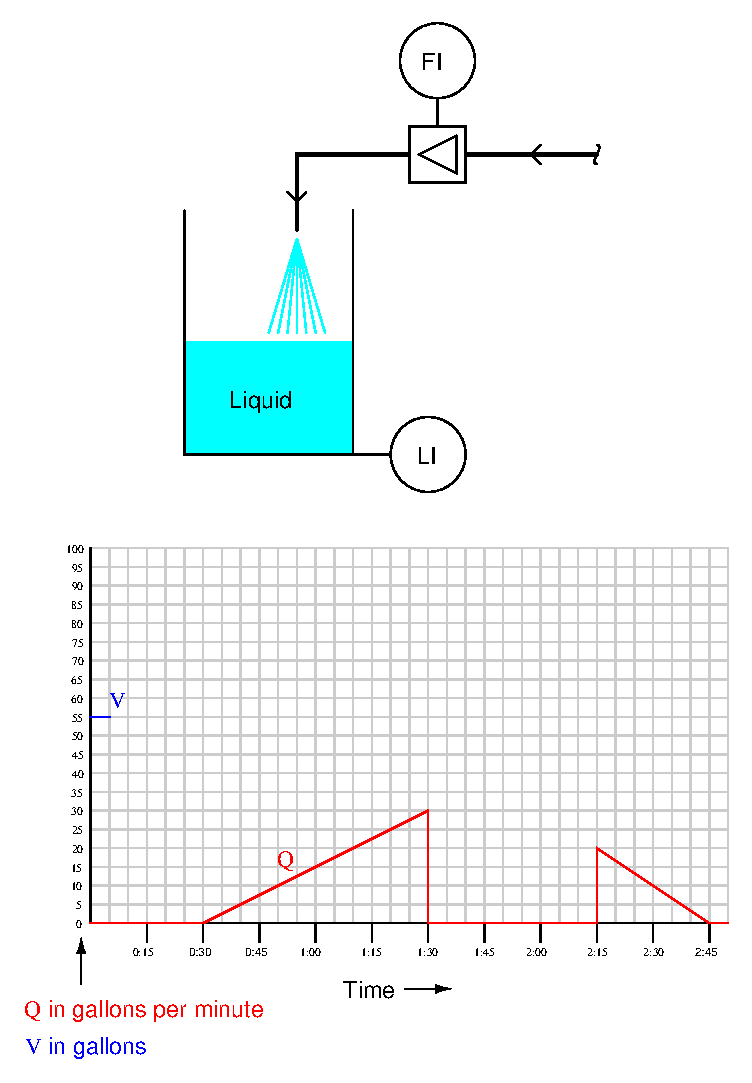
\includegraphics[width=15.5cm]{i01581x01.eps}$$

\begin{itemize}
\item{} Tid = 0:15; Volum = \underbar{\hskip 50pt}
\vskip 5pt
\item{} Tid = 1:30; Volum = \underbar{\hskip 50pt}
\vskip 5pt
\item{} Tid = 1:45; Volum = \underbar{\hskip 50pt}
\vskip 5pt
\item{} Tid = 2:45; Volum = \underbar{\hskip 50pt}
\end{itemize} 
 
Som angitt i grafen inneholder tanken 55 gallon væske ved tid = 0:00. Merk at tidsenheten på grafens horisontale akse er minutter:sekunder, ikke timer:minutter.

\vskip 10pt

Beregn også akkumulert volum i lagringstanken ved tid = 1:00 og tid = 2:30. Bruk denne informasjonen til å skissere en graf for akkumulert væskevolum over tid.

\vskip 20pt \vbox{\hrule \hbox{\strut \vrule{} {\bf Forslag til sokratisk diskusjon} \vrule} \hrule}

\begin{itemize}
\item{} Hvis du sto ved røret som slipper vann inn i denne tanken, hvordan ville væskestrømmen i grafen {\it sett ut}? Ville strømmen variert over tid, eller holdt seg jevn? Ville den startet og stoppet, eller vært kontinuerlig?
\item{} Anta at du fikk en graf for vannvolum i tanken og ble bedt om å beregne strømningsrate inn i eller ut av tanken. Hvilket prinsipp fra kalkulus ville du brukt for å løse oppgaven?
\item{} Anta at strømningsraten ($Q$) i grafen representerte strøm {\it ut} av tanken i stedet for strøm {\it inn} i tanken. Hvordan ville denne forskjellen påvirket formen på $V$-grafen?
\item{} En tank som fylles med vann kan sammenlignes med en elektrisk kondensator som ``fylles'' med ladning. Identifiser passende variabler for en graf som viser ``fyllingen'' av en kondensator.
\end{itemize}

\underbar{file i01581}
%(END_QUESTION)





%(BEGIN_ANSWER)

\begin{itemize}
\item{} Tid = 0:15; Volum = 55 gallon
\item{} Tid = 1:30; Volum = 70 gallon
\item{} Tid = 1:45; Volum = 70 gallon
\item{} Tid = 2:45; Volum = 75 gallon
\end{itemize} 

\begin{itemize}
\item{} Tid = 1:00; Volum = 58.75 gallon
\item{} Tid = 2:30; Volum = 73.75 gallon
\end{itemize} 

$$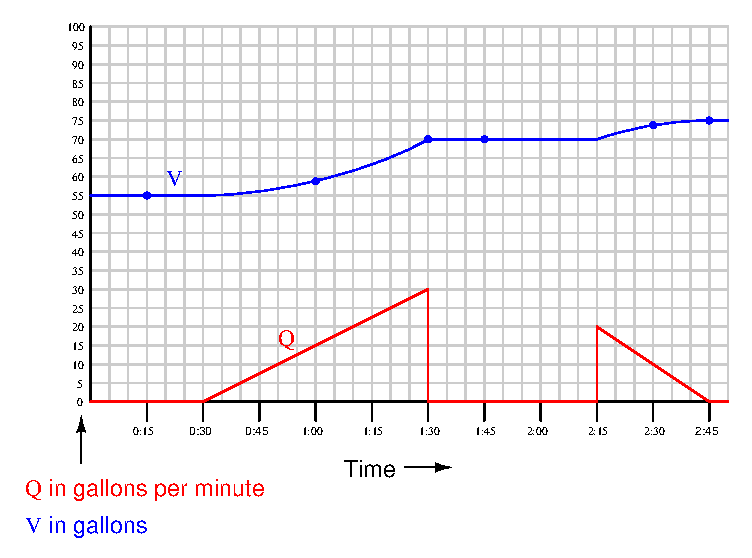
\includegraphics[width=15.5cm]{i01581x02.eps}$$

%(END_ANSWER)





%(BEGIN_NOTES)




\vskip 20pt \vbox{\hrule \hbox{\strut \vrule{} {\bf Forslag til sokratisk diskusjon} \vrule} \hrule}

\begin{itemize}
\item{} Foreslå en annen flowtrend for studentene (for eksempel en annen trendprofil), og la dem forutsi hvordan volumtrenden endres.
\item{} Foreslå en annen volumtrend for studentene (for eksempel en annen trendprofil), og la dem forutsi hvilken flowprofil som må til for å skape den.
\end{itemize}


%INDEX% Mathematics, calculus: integral (accumulated volume as the integral of flow)

%(END_NOTES)
